\documentclass[a4paper,11pt]{article}
\usepackage[T1]{fontenc}
\usepackage[utf8]{inputenc}
\usepackage{lmodern}
\usepackage{graphicx}

\title{Neural network notes}
\author{Marco Marini}

\begin{document}

\maketitle
\tableofcontents

\begin{abstract}
Studio del gioco wall
\end{abstract}

\section{Generale}

Wall è un gioco dove una pallina si muove in un campo rettangolare con traiettorie rettilinee diagonali.
I limiti superiore e laterali sono costituiti da muri che
fanno rimbalzare la pallina.
La parte inferiore invece è aperta e una racchetta controllata dal giocatore si muove orizzontalmente
permettendo allo stesso di far rimbalzare la pallina all'interno del campo da gioco.
La numerazione delle righe parte dal basso e verso l'alto.

$
\begin{array}{ccccccccccccccc}
=	& = & = & = & = & = & = & = & = & = & = & = & = & = & = \\
|	&  &  &  &  &  &  &  &  &  &  &  &  &  & | \\ 
|	&  &  &  &  &  &  &  &  &  &  &  &  &  & | \\ 
|	&  &  &  &  &  &  &  &  &  &  &  &  &  & | \\ 
|	&  &  &  &  &  &  &  &  &  &  &  &  &  & | \\ 
|	&  &  &  &  &  &  &  &  &  &  &  &  &  & | \\ 
|	&  &  &  &  &  & O &  &  &  &  &  &  &  & | \\ 
|	&  &  &  &  &  &  &  &  &  &  &  &  &  & | \\ 
|	&  &  &  &  &  &  &  &  &  &  &  &  &  & | \\ 
|	&  &  &  &  &  &  &  &  &  &  &  &  &  & | \\ 
	&  &  & = & = & = &  &  &  &  &  &  &  &  & 
\end{array} 
$

Definiamo 
\[ n = 10 \] il numero di righe del campo
\[ m = 13 \] il numero di colonne
\[ w = 3 \] la larghezza della racchetta


\section{Spazio degli stati}

In un qualsiasi momento lo stato del gioco è rappresentato dalla posizione
della pallina, la direzione di spostamento della pallina e la posizione della racchetta.
Calcoliamo il numero di stati possibili:

La racchetta può trovarsi in uno degli
\[m - w + 1 = 11 \] possibili posizioni.

\subsection{Palla in centro}

Quando la pallina non si trova in prossimità dei muri o della racchetta
può muoversi in 4 diverse direzioni: NE, SE, SO, NO.
Quindi abbiamo
\[ 4 (n-2)(m-2) (m - w + 1) = 3872 \]
possibili stati.

\subsection{Palla negli angoli superiori}

Negli angoli superiori la pallina può avere solo una direzione (NO per l'angolo ovest e NE per l'angolo est) quindi
si aggiungono altri 
\[
	2 (m - w +1) = 11
\] stati.

\subsection{Palla nel muro superiore}

Quando si trova in prossimità invece del muro superiore può avere solo due direzioni (NE o NO) quindi \[ (m - w + 1) 2 (m - 2) = 242 \] stati

\subsection{Palla nei muri laterali}

Quando si trova in prossimità invece del muro laterali, la pallina può assumere solo due possibili velocità (SE NE per il lato est e SO NO per il lato ovest) quindi avremo \[ 2 (m - w + 1) 2 (n - 2) = 352 \] ulteriori stati.


\section{Rimbalzi certi}

Contiamo ora quanti stati che generano premi positivi indipendentemente dalla strategia.

La racchetta si trova completamente a sx, la pallina può trovarsi completamente a sx con solo la direzione NE possibile, oppure si può trovare nelle due colonne successive con direzioni NO o NE, oppure in quarta colonna con direzione NO
\[ 1 + 2(w-1) + 1 = 2w =  6 \]
possibili stati.

Simmetricamente abbiamo altri 6 stati quando la racchetta si trova completamente a dx.

La racchetta si trova tra la seconda colonna e la quartultima colonna, la pallina può trovarsi nelle tre colonne successive con direzioni NO o NE
\[
2w(m-w-2) = 48
\]
possibili stati.

In tutto possiamo contare 
\[
4w+2w(m-w-2) = 2w(m-w)=60
\]
possibili stati di rimbalzo certo.


\section{Fine gioco}

Contiamo ora quanti stati dove, indipendentemente dalla strategia, si arriva a fine gioco.

Quando la racchetta si trova in prima colonna e la pallina si trova in quarta o quinta colonna con direzione SE o dalla sesta alla penultima colonna con due direzioni possibili o infine la pallina si trova in ultima colonna direzione SO
\[
2(m-w-3)+3=2(m-w)-3=17
\]
stati possibili.

Quando la racchetta si trova in seconda colonna e la pallina si trova in quinta o sesta colonna con direzione SE oppure tra la settima e la penultima colonna con due direzioni possibili o infine la pallina si trova in ultima colonna con direzione SO
\[
2(m-w-4)+3 = 2(m-w)-5 = 15
\]
stati possibili.

Quando la racchetta si trova in terza colonna e la pallina si trova in seconda colonna con direzione SO o in sesta o settima colonna con direzione SE oppure tra la ottava e la penultima colonna con due direzioni possibili o infine la pallina si trova in ultima colonna con direzione SO
\[
2(m-w-5)+4= 2(m-w)-6 = 14
\]
stati possibili.

Gli stessi stati li abbiamo per simmetria quando la racchetta si trova al lato opposto.

Quando la racchetta si trova tra la quarta colonna e sei colonne prima dell'ultima e la pallina si trova nei bordi con singole direzioni, o nelle due adiacenti la sx o la dx della racchetta con singole direzioni o nelle colonne intermedie tra i bordi e le precedenti colonne con due direzioni
\[
2(m-w-6)+6 = 2(m-w)-6=14
\]

In tutto quindi ci sono
\[
\begin{array}{r}
 2[2(m-w)-3+2(m-w)-5+2(m-w)-6]+2(m-w)-6 = \\
 = 12(m-w)-28+2(m-w)-6 = \\
 = 14(m-w)-34 = 106 \\
\end{array}
\] stati di fine certa del gioco.

\section{Rimbalzi condizionali}

Contiamo ora gli stati di rimbalzo dipendenti dalla strategia.

Quando la racchetta si trova in prima colonna e la pallina in quinta colonna con direzione SO 
\[
1
\]
stato possibile.

Quando la racchetta si trova in seconda colonna e la pallina in prima colonna con direzione SE o in quinta o sesta colonna con direzione SO
\[
3
\]
stati possibili.

Altrettanti stati per simmetria.

Quando la racchetta si trova tra la terza e cinque colonne prima dell'ultima, la pallina nelle due colonne antecedente la racchetta
con direzione SE o nelle duce colonne sucessiva la fine della racchetta
con direzione S0
\[
4 (m-w-4)=4(m-w)-16=24
\]

In totale abbiamo
\[
(1+3)2+4(m-w)-16=4(m-w)-8=32
\]
possibili stati.

\section{Miglior policy}

La policy migliore è quella di far rimbalzare la pallina una volta che raggiunge la parte inferiore del campo

La pallina rimbalza ogni
\[
2 (n - 1)
\]
passi.

Il ritorno aspettato allo stato dopo $ i = (1 \dots 2(n-1) $ passi dal rimbalzo sarà quindi
\[
R_i = \gamma ^ {2(n-1)-i} \sum_{j=0}^{\infty} R^+ \gamma ^ {2(n-1)j} =
R^+ \frac{ \gamma ^ {2(n-1)-i}}{1-\gamma ^ {2(n-1)}}
\]


\section{Considerazioni}

Consideriamo ora la startegia $ \varepsilon $-greedy dove viene generata un'azione casuale con probabilità $ \varepsilon $.

Supponiamo che l'azione casuale porti alla fine gioco.

Che probabilità abbiamo che la sequenza si concluda con la fine del gioco dopo $ k $ iterazioni?

\[
P(fine) = 1 - (1 - \varepsilon) ^ k
\]

Per una sequenza di episodica abbiamo che \[ k = 2(n-1) \] quindi
\[
P(fine) = 1 - (1 - \varepsilon) ^ {2(n-1)}
\]

Quindi se vogliamo che la fine del gioco capiti con probabilità $ p $ sobbiamo avere
\[
\varepsilon = 1- (1 - p) ^ \frac{1}{2(n-1)}
\]

nel caso di $ p = 0.1 $ avremo che 
\[
\varepsilon \approx 5.8363 \cdot 10^{-3}
\]

In tutto gli stati finali sono quindi 
\[
\begin{array}{r}
 2w(m-w)+14(m-w)-34+4(m-w)-8= \\
 =2w(m-w)+18(m-w)-42= \\
 =2(w+9)(m-w)-42= 198\\
\end{array}
\]

Supponiamo ora che la strategia porti ad una distribuzione uniforme degli stati i rimbalzo, abbiamo quindi tre situazioni:

\begin{itemize}
	\item 	
	Rimbalzo certo con probabilità
	 \[ P(rimbalzo)=\frac{2w(m-w)}{2(w+9)(m-w)-42}
	 =\frac{w(m-w)}{(w+9)(m-w)-21}
	 = \frac{10}{33}\approx0.303
	 \]

	\item 	
	Finale certo con probabilità 
	 \[ P(fine)=\frac{14(m-w)-34}{2(w+9)(m-w)-42}
	 =\frac{7(m-w)-17}{(w+9)(m-w)-21}
	 = \frac{53}{99}\approx0.535
	 \]
	 
	 \item 	
	 Rimbalzo condizionato con probabilità 
	 \[ P(condizionale)=\frac{4(m-w)-8}{2(w+9)(m-w)-42}
	 =2\frac{(m-w)-2}{(w+9)(m-w)-21}
	 = \frac{16}{99}\approx0.162
	 \]
\end{itemize}

\section{Batch critic}

Per migliorare l'apprendimento della componente critic si 
applica l'algoritmo di apprendimento in maniera iterativa su un sottoinsieme limitato delle ultime esperienze (SARS stato iniziale, azione, premio, stato finale) parallelamente all'algoritmo di apprendimento on-line.

Il grafico sottostante rappresenta la lunghezza media degli episodi nel gioco del muro nei casi dell'algoritmo puramente on line e
di quello batch dove l'interazione viene ritardata di 0, 200, 600 millisecondi per permettere l'apprendimento.

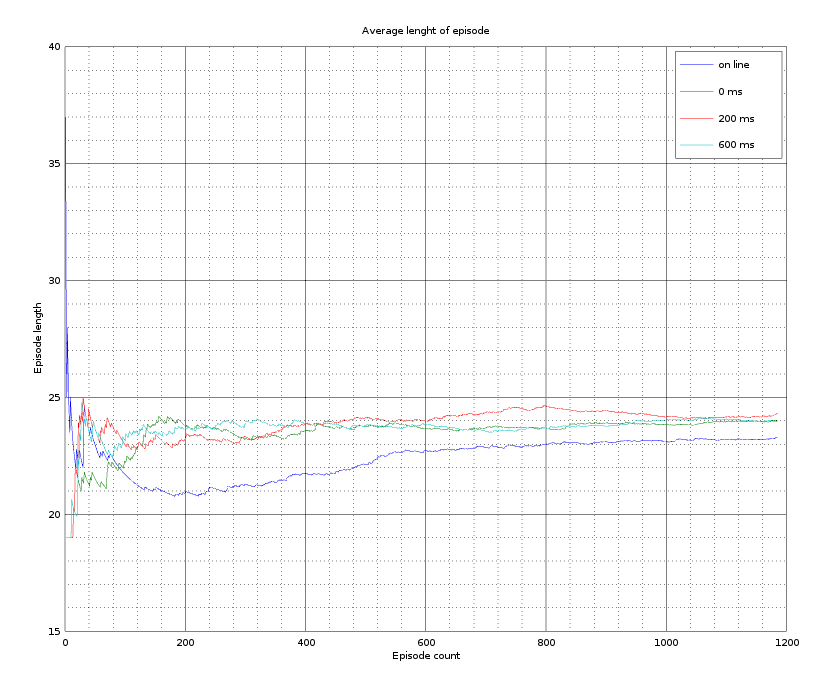
\includegraphics[width=300pt]{episodes}

Si può notare che dopo per un numero sufficiente di episodi l'algoritmo batch ha tende ad essere leggermente migliore di quello on line e che la differenza tra i vari tempi di ritardo non è particolarmente significativa.


\end{document}
